\documentclass[11pt, oneside, a4paper]{article}

%--- PREAMBLE ---%
\usepackage{geometry}
\usepackage[utf8]{inputenc}
\usepackage[T1]{fontenc}
\usepackage{hyperref}
\usepackage{float}
\usepackage{amsmath}
\usepackage{pgfplots}
\pgfplotsset{width=10cm,compat=1.9}

\setcounter{tocdepth}{2}
\hypersetup{
	hidelinks
}

\title{CMPE 300: Project 1}
\author{
	Name1 Surname1\\StudentNumber1
	\and
	Name2 Surname2\\StudentNumber2
}
\date{\today}

%-- DOCUMENT ---%

\begin{document}
	\maketitle

	\tableofcontents

	\newpage

	\section{Theoretical Analysis}

	\subsection{Basic operation is the comparison marked as (1)}

	\subsubsection{Analysis of B(n)}

	\subsubsection{Analysis of W(n)}

	\subsubsection{Analysis of A(n)}

	\subsection{Basic operations are the two loop increments marked as (2)}

	\subsubsection{Analysis of B(n)}

	\subsubsection{Analysis of W(n)}

	\subsubsection{Analysis of A(n)}

	\subsection{Basic operations are the four assignments marked as (3)}

	\subsubsection{Analysis of B(n)}

	\subsubsection{Analysis of W(n)}

        \subsubsection{Analysis of A(n)}

	\subsection{Basic operations are the four assignments marked as (4)}

	\subsubsection{Analysis of B(n)}

	\subsubsection{Analysis of W(n)}
	
        \subsubsection{Analysis of A(n)}

	\section{Identification of Basic Operation(s)}

	Here, state clearly which operation(s) in the algorithm must be the basic operation(s). Also, you should provide a simple explanation about why you have decided on the basic operation you choose. (1-3 sentences)

	\section{Real Execution}

	\begin{table}[H]
		\centering
		\begin{tabular}{|l|l|} \hline
			\textbf{N Size} & \textbf{Time Elapsed} \\ \hline
			1 & ??? \\ \hline
			5 & ??? \\ \hline
			10 & ??? \\ \hline
			20 & ??? \\ \hline
			30 & ??? \\ \hline
			40 & ??? \\ \hline
			50 & ??? \\ \hline
			60 & ??? \\ \hline
			70 & ??? \\ \hline
			90 & ??? \\ \hline
			100 & ??? \\ \hline
			120 & ??? \\ \hline
			130 & ??? \\ \hline
			140 & ??? \\ \hline
			150 & ??? \\ \hline
			160 & ??? \\ \hline
			170 & ??? \\ \hline
		\end{tabular}
		\caption{Best Case Real Execution Times}
		\label{tab:best-case}
	\end{table}


	\begin{table}[H]
		\centering
		\begin{tabular}{|l|l|} \hline
			\textbf{N Size} & \textbf{Time Elapsed} \\ \hline
			1 & ??? \\ \hline
			5 & ??? \\ \hline
			10 & ??? \\ \hline
			20 & ??? \\ \hline
			30 & ??? \\ \hline
			40 & ??? \\ \hline
			50 & ??? \\ \hline
			60 & ??? \\ \hline
			70 & ??? \\ \hline
			90 & ??? \\ \hline
			100 & ??? \\ \hline
			120 & ??? \\ \hline
			130 & ??? \\ \hline
			140 & ??? \\ \hline
			150 & ??? \\ \hline
			160 & ??? \\ \hline
			170 & ??? \\ \hline
		\end{tabular}
		\caption{Worst Case Real Execution Times}
		\label{tab:worst-case}
	\end{table}

	\begin{table}[H]
		\centering
		\begin{tabular}{|l|l|} \hline
			\textbf{N Size} & \textbf{Time Elapsed} \\ \hline
			1 & ??? \\ \hline
			5 & ??? \\ \hline
			10 & ??? \\ \hline
			20 & ??? \\ \hline
			30 & ??? \\ \hline
			40 & ??? \\ \hline
			50 & ??? \\ \hline
			60 & ??? \\ \hline
			70 & ??? \\ \hline
			90 & ??? \\ \hline
			100 & ??? \\ \hline
			120 & ??? \\ \hline
			130 & ??? \\ \hline
			140 & ??? \\ \hline
			150 & ??? \\ \hline
			160 & ??? \\ \hline
			170 & ??? \\ \hline
		\end{tabular}
		\caption{Average Case Real Execution Times}
		\label{tab:avg-case}
	\end{table}

	\section{Comparison}

	\subsection{Best Case}

	\subsubsection{Graph of the real execution time of the algorithm}

	% Here is an example line plot of data points for you. Feel free to change it or use something else.

	\begin{figure}[H]
	\centering
	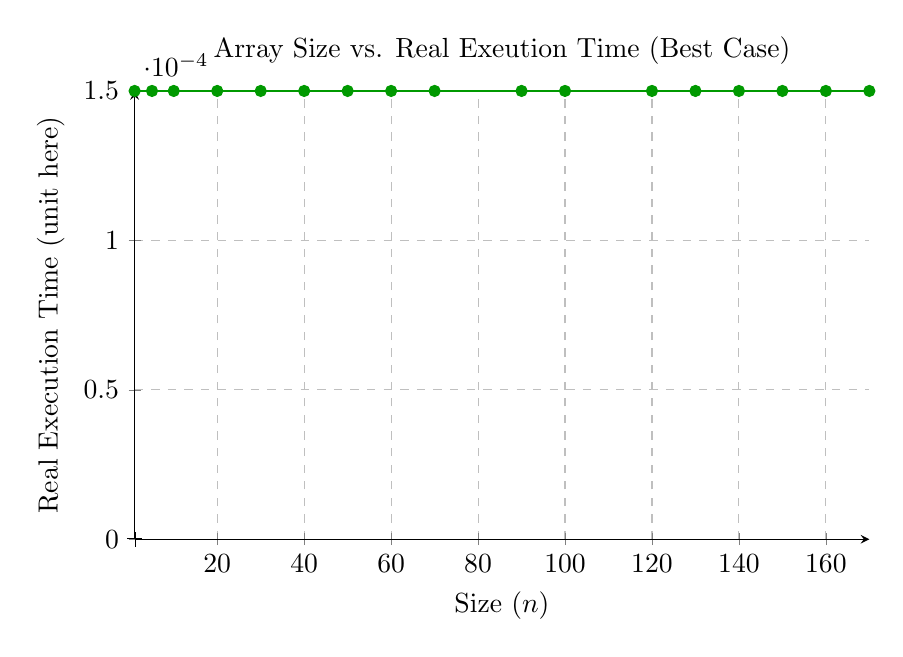
\begin{tikzpicture}
		\begin{axis}[
			% Axis labels and title
			title={Array Size vs. Real Exeution Time (Best Case)},
			xlabel={Size (\(n\))},
			ylabel={Real Execution Time (unit here)},
			% Axis limits
			%xmin=0, xmax=100,
			ymin=0, %ymax=200,
			% Axis ticks
			% xtick={0,20,40,60,80,100},
			% ytick={0,20,40,60,80,100,120},
			grid=both,
			axis lines=left,
			axis line style={|-stealth},
			grid style=dashed,
			width=0.9\textwidth,
			height=\axisdefaultheight
			]
			\addplot[
				color=green!60!black,
				mark=*,
				smooth
				]
			% Change the coordinates here with your own data:
			coordinates {
				(1,   0.00015)
				(5,   0.00015)
				(10,  0.00015)
				(20,  0.00015)
				(30,  0.00015)
				(40,  0.00015)
				(50,  0.00015)
				(60,  0.00015)
				(70,  0.00015)
				(90,  0.00015)
				(100, 0.00015)
				(120, 0.00015)
				(130, 0.00015)
				(140, 0.00015)
				(150, 0.00015)
				(160, 0.00015)
				(170, 0.00015)
			};
		\end{axis}
	\end{tikzpicture}
	\end{figure}

	\subsubsection{Graph of the theoretical analysis when basic operation is the operation marked as (1)}

	\subsubsection{Graph of the theoretical analysis when basic operation is the operation marked as (2)}

	\subsubsection{Graph of the theoretical analysis when basic operation is the operation marked as (3)}

	\subsubsection{Graph of the theoretical analysis when basic operation is the operation marked as (4)}


	\subsubsection{Comments}



	\subsection{Worst Case}

	\subsubsection{Graph of the real execution time of the algorithm}

	\subsubsection{Graph of the theoretical analysis when basic operation is the operation marked as (1)}

	\subsubsection{Graph of the theoretical analysis when basic operation is the operation marked as (2)}

	\subsubsection{Graph of the theoretical analysis when basic operation is the operation marked as (3)}

	\subsubsection{Graph of the theoretical analysis when basic operation is the operation marked as (4)}

	\subsubsection{Comments}




	\subsection{Average Case}

	% Graph of the real execution time of the algorithm
	
	\subsubsection{Graph of the theoretical analysis when basic operation is the operation marked as (1)}

	\subsubsection{Graph of the theoretical analysis when basic operation is the operation marked as (2)}

	\subsubsection{Graph of the theoretical analysis when basic operation is the operation marked as (3)}

	\subsubsection{Graph of the theoretical analysis when basic operation is the operation marked as (4)}

	\subsubsection{Graph of the theoretical analysis when basic operation is the operation marked as (5)}

	\subsubsection{Comments}

\end{document}
